%============================================================================%
%
%	DOCUMENT DEFINITION
%
%============================================================================%

%we use article class because we want to fully customize the page and dont use a cv template
\documentclass[10pt,A4]{article}	

% Include document definitions


%----------------------------------------------------------------------------------------
%	ENCODING
%----------------------------------------------------------------------------------------

%we use utf8 since we want to build from any machine
\usepackage[utf8]{inputenc}		

%-------------------------------------------------------------------------------
%	LOGIC
%-------------------------------------------------------------------------------


% provides \isempty test
\usepackage{xifthen}

%-------------------------------------------------------------------------------
%	FONT
%-------------------------------------------------------------------------------


% some tex-live fonts - choose your own

% \usepackage[defaultsans]{droidsans}
% \usepackage[default]{comfortaa}
% \usepackage{cmbright}
% \usepackage[default]{raleway}
% \usepackage{fetamont}
\usepackage[default]{gillius}
% \usepackage[light,math]{iwona}
% \usepackage[thin]{roboto} 

% set font default
\renewcommand*\familydefault{\sfdefault} 	
\usepackage[T1]{fontenc}

% more font size definitions
\usepackage{moresize}		

\usepackage{fontawesome}

%-------------------------------------------------------------------------------
%	PAGE LAYOUT  DEFINITIONS
%-------------------------------------------------------------------------------


%debug page outer frames
%\usepackage{showframe}			


%define page styles using geometry
\usepackage[a4paper]{geometry}		

% for example, change the margins to 2 inches all round
\geometry{top=1cm, bottom=-.6cm, left=0.4cm, right=1cm} 	


%less space between header and content
\setlength{\headheight}{-5pt}		


%customize entries left, center and right
%\lhead{}
%\chead{ \small{Jan Küster  $\cdot$ Consultant and Software Engineer $\cdot$  Bremen, Germany  $\cdot$  \textcolor{sectcol}{\textbf{info@jankuester.com}}  $\cdot$ +49 176 313 *** **}}
%\rhead{}


%indentation is zero
\setlength{\parindent}{0mm}

%-------------------------------------------------------------------------------
%	TABLE /ARRAY DEFINITIONS
%-------------------------------------------------------------------------------

%for layouting tables
\usepackage{multicol}			
\usepackage{multirow}

%extended aligning of tabular cells
\usepackage{array}

\newcolumntype{x}[1]{{\raggedleft\hspace{0pt}}p{#1}}%


%-------------------------------------------------------------------------------
%	GRAPHICS DEFINITIONS
%-------------------------------------------------------------------------------

%for header image
\usepackage{graphicx}

%for floating figures
\usepackage{wrapfig}
\usepackage{float}
%\floatstyle{boxed} 
%\restylefloat{figure}

%for drawing graphics		
\usepackage{tikz}				
\usetikzlibrary{shapes, backgrounds,mindmap, trees}


%-------------------------------------------------------------------------------
%	Color DEFINITIONS
%-------------------------------------------------------------------------------
 
\usepackage{transparent}
\usepackage{color}

%accent color
\definecolor{complcol}{RGB}{250,150,10}

%dark background color
\definecolor{bgcol}{RGB}{110,110,110}

%light background / accent color
\definecolor{softcol}{RGB}{225,225,225}

\definecolor{sectcol}{RGB}{0,120,150}


%Package for links, must be the last package used
\usepackage[colorlinks, urlcolor=blue]{hyperref}

%============================================================================%
%
%
%	DEFINITIONS
%
%
%============================================================================%

% returns minipage width minus two times \fboxsep
% to keep padding included in width calculations
\newcommand{\mpwidth}{\linewidth-\fboxsep-\fboxsep}
	

%-------------------------------------------------------------------------------
% 	ARROW GRAPHICS in Tikz
%-------------------------------------------------------------------------------

% a six pointed arrow poiting to the left
\newcommand{\tzlarrow}{(0,0) -- (0.2,0) -- (0.3,0.2) -- (0.2,0.4) -- (0,0.4) -- (0.1,0.2) -- cycle;}	

% include the left arrow into a tikz picture
% param1: fill color
%
\newcommand{\larrow}[1]
{\begin{tikzpicture}[scale=0.58]
	 \filldraw[fill=#1!100,draw=#1!100!black]  \tzlarrow
 \end{tikzpicture}
}

% a six pointed arrow poiting to the right
\newcommand{\tzrarrow}{ (0,0.2) -- (0.1,0) -- (0.3,0) -- (0.2,0.2) -- (0.3,0.4) -- (0.1,0.4) -- cycle;}

% include the right arrow into a tikz picture
% param1: fill color
%
\newcommand{\rarrow}
{
\begin{tikzpicture}[scale=0.7]
	\filldraw[fill=sectcol!100,draw=sectcol!100!black] \tzrarrow
 \end{tikzpicture}
}

%-------------------------------------------------------------------------------
%	custom sections
%-------------------------------------------------------------------------------

% create a coloured box with arrow and title as cv section headline
% param 1: section title
%
\newcommand{\cvsection}[1]
{
\colorbox{sectcol}{\mystrut \makebox[1\mpwidth][l]{
\larrow{bgcol} \hspace{-8pt} \larrow{bgcol} \hspace{-8pt} \larrow{bgcol} \textbf{\textcolor{white}{\uppercase{#1}}}\hspace{4pt}
}}\\
}

% create a coloured arrow with title as cv meta section section
% param 1: meta section title
%
\newenvironment{metasection}[1] {
	\vspace{6pt}
	\begin{center}
		\textcolor{white}{\large{\uppercase{#1}}}\\
	\normalsize
	\parbox{0.7\mpwidth}{\textcolor{white}	\hrule}
}{\end{center}}


%-------------------------------------------------------------------------------
%	 CV EVENT
%-------------------------------------------------------------------------------

% creates a stretched box as cv entry headline followed by some paragraphs about 
% the work you did
% param 1:	event time i.e. 2014 or 2011-2014 etc.
% param 2:	event name (what did you do?)
% param 3:	institution (where did you work / study)
% param 4:	list of paragraphs outlining your contributions, see example usage below
%
\newcommand{\cvevent}[4]
{
	\vspace{6pt}
		\begin{tabular*}{1\mpwidth}{p{0.55\mpwidth} >{\raggedleft\arraybackslash}p{0.42\mpwidth}}
			\textcolor{black}{\textbf{#2}} & \textcolor{complcol}{#3}, \textcolor{bgcol}{#1} 
		\end{tabular*}
\vspace{0pt}
\textcolor{softcol}{\hrule}
\vspace{6pt}
	\cvlist{#4}
\vspace{0pt}
}

% Same as \cvevent, but without the institution field and more compact
\newcommand{\cvline}[2]
{
\vspace{4pt}
	\begin{tabular*}{1\mpwidth}{p{0.8\mpwidth} x{0.18\mpwidth}}
 	\textcolor{black}{\cvlist {#2}} & \textcolor{bgcol}{	#1} 
	\end{tabular*}
\vspace{0pt}
\textcolor{softcol}{\hrule}
}

% formats a list of strings with variable length for use in `\cvevent`
% param 1: a list of strings outlining your contributions
\newcommand{\cvlist}[1] {
    \foreach \listitem in {#1}
    {
        \begin{tabular*}
            {1\mpwidth}{p{1\mpwidth}}
            \parbox{1\mpwidth}{\larrow{softcol} \listitem}
            \vspace{2pt}
        \end{tabular*}
    }
}

% creates a stretched box as 
\newcommand{\cveventmeta}[2]
{
	\mbox{\mystrut \hspace{87pt}\textit{#1}}\\
	#2
}

%-------------------------------------------------------------------------------
% CUSTOM STRUT FOR EMPTY BOXES
%-------------------------------------------------------------------------------

\newcommand{\mystrut}{\rule[-.3\baselineskip]{0pt}{\baselineskip}}

%-------------------------------------------------------------------------------
% CUSTOM LOREM IPSUM
%-------------------------------------------------------------------------------
\newcommand{\lorem}
{Lorem ipsum dolor sit amet, consectetur adipiscing elit. Donec a diam lectus.}


% use to vertically center content
% credits to: http://tex.stackexchange.com/questions/7219/how-to-vertically-center-two-images-next-to-each-other
\newcommand{\vcenteredinclude}[1]{\begingroup
\setbox0=\hbox{\includegraphics{#1}}%
\parbox{\wd0}{\box0}\endgroup}

% use to vertically center content
% credits to: http://tex.stackexchange.com/questions/7219/how-to-vertically-center-two-images-next-to-each-other
\newcommand*{\vcenteredhbox}[1]{\begingroup
\setbox0=\hbox{#1}\parbox{\wd0}{\box0}\endgroup}

%-------------------------------------------------------------------------------
%	ICON-SET EMBEDDING
%------------------------------------------------------------------------------ 

% at this point we simplify our icon-embedding by simply referring to a set of png images.
% if you find a good way of including svg without conflicting with other packages you can
% replace this part
\newcommand{\icon}[3]{
	\makebox(#2, #2){\textcolor{#3}{\csname fa#1\endcsname}}
}	%icon shortcut
\newcommand{\icontext}[4]{ 						%icon with text shortcut
	\vcenteredhbox{\icon{#1}{#2}{#4}} \vcenteredhbox{\textcolor{#4}{#3}}
}
\newcommand{\iconhref}[5]{ 						%icon with website url
    \vcenteredhbox{\icon{#1}{#2}{#5}} \href{#4}{\textcolor{#5}{#3}}
}

\newcommand{\iconemail}[5]{ 						%icon with email link
    \vcenteredhbox{\icon{#1}{#2}{#5}} \href{mailto:#4}{\textcolor{#5}{#3}}
}

\newcommand{\customicon}[3]{
	\makebox(#2, #2){\textcolor{#3}{\csname \includegraphics*[width=#2pt, height=#2pt]{#1}\endcsname}}
}	% Custom icon shortcut (#1 is the icon path)

\newcommand{\customicontext}[4]{ %icon with text shortcut
	\vcenteredhbox{\customicon{#1}{#2}{#4}} \vcenteredhbox{\textcolor{#4}{#3}}
}

%============================================================================%
%
%	DOCUMENT CONTENT
%
%============================================================================%
\begin{document}
\fcolorbox{white}{white}{\begin{minipage}[c][0.95\textheight][t]{0.80\linewidth}

%-------------------------------------------------------------------------------
%	TITLE HEADLINE
%-------------------------------------------------------------------------------

\vspace{-3pt}
% use this for multiple words like working titles etc.
%\hspace{-0.25\linewidth}\colorbox{bgcol}{\makebox[1.5\linewidth][c]{\hspace{46pt}\HUGE{\textcolor{white}{\uppercase{M.Sc. Jan Küster}} } \textcolor{sectcol}{\rule[-1mm]{1mm}{0.9cm}} \parbox[b]{5cm}{   \large{ \textcolor{white}{{IT Consultant}}}\\
% \large{ \textcolor{white}{{JS Fullstack Engineer}}}}
%}}

% use this for single words, e.g. CV or RESUME etc.
\colorbox{bgcol}{\makebox[\mpwidth][c]{\Large{\textcolor{white}{\uppercase{Francesco Ioli}} } \textcolor{sectcol}{\rule[-1mm]{1mm}{0.9cm}} \RESUME{\textcolor{white}{\uppercase{CV}} } }}

%-------------------------------------------------------------------------------
%	HEADER IMAGE
%-------------------------------------------------------------------------------

%\hspace{-1.6cm}
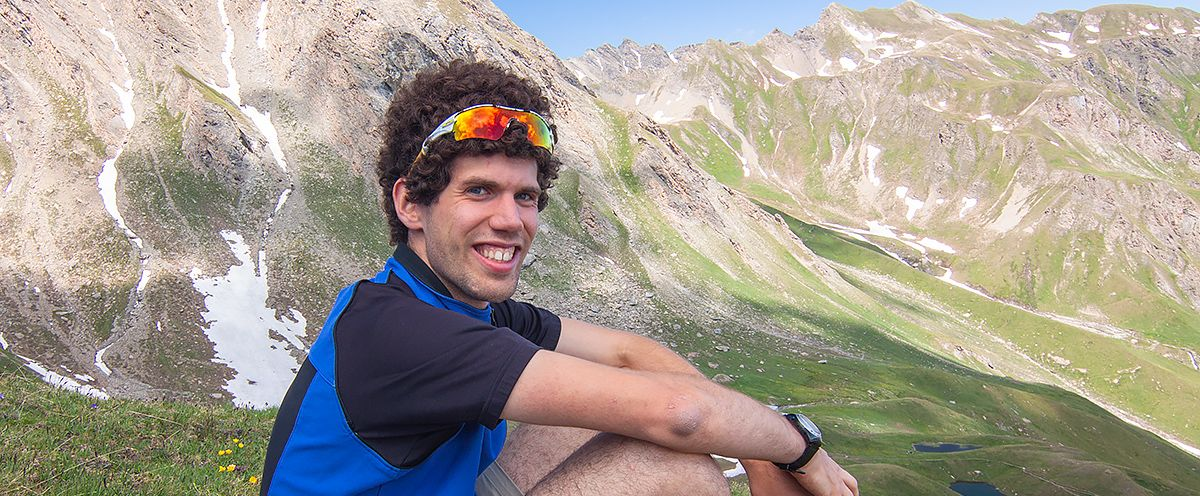
\includegraphics[trim= 150 150 0 60, clip,width=\linewidth]{img/img_montagna.jpg}	%trimming relative to image size
% [trim={left bottom right top},clip]

%-------------------------------------------------------------------------------
%	SUMMARY
%-------------------------------------------------------------------------------
\transparent{0.85}%
\vspace{-100pt}
\hspace{0.5\linewidth}
\colorbox{bgcol}{
	\parbox{0.45\linewidth}{
		\transparent{1}%
		\begin{center}
		% \larrow{sectcol}\larrow{sectcol}
		\textcolor{white}{I am a PhD student in Geomatics with a focus on photogrammetry and 3D reconstruction. I'm working on low-cost stereo-cameras and UAV SfM for glacier monitoring. 
		I am a UAV pilot, licensed to operate in critical scenarios.}
		\end{center}
	}
}
\vspace{30pt}

%-------------------------------------------------------------------------------
%	EXPERIENCE
%-------------------------------------------------------------------------------

\cvsection{Experience}
%\textcolor{softcol}{\hrule}

\cvevent{2020 - now}{PhD Student}{Politecnico di Milano, DICA}
	{My research focusees on UAV-based and terrestial photogrammetry for land and infrastructure monitoring. I am working on a low-cost image-based system for 4D glacier monitoring (\href{https://github.com/franioli/icepy4d}{ICEpy4D}) and on UAV-photogrammetry for structural health assessment and crack detection on concrete bridges.
	}

\cvevent{2022}{Visiting PhD student}{University of Twente, ITC}{
	Developing a wide-baseline stereo matching workflow with Deep Learning for 4D monitoring of an alpine glacier by using low-cost time-lapse cameras.
	}

\cvevent{2020 - now}{Teaching assistant}{Politecnico di Milano}{
	\textit{Course of Trattamento delle Osservazini} (Statistics) [2020{,} 2021{,} 2022],
	\textit{Course of Sistemi Informativi Territoriali} (GIS) [2020{,} 2021],
	\textit{Course of Tecniche di rilievo e modellazione 3D per l'architettura} (3D modelling for architecture) [2020{,} 2021{,} 2022].
	}

\cvevent{2021 - 2022}{Tutoring}{Politecnico di Milano}{Tutor for the Summer School \textit{Design and Execution of Topographic Surveys for Land Monitoring} at the Belvedere Glacier (Italian Alps) aimed at introducing BSc and MSc students to topographic fielworks in mountain environments.
}

\vspace{12pt}

%-------------------------------------------------------------------------------
%	EDUCATION SECTION
%-------------------------------------------------------------------------------
\cvsection{Education}

\cvevent{2017 - 2020}{MSc in Environmental and
Land Planning Engineering}{Politecnico di Milano}{Major in Land Monitoring and Diagnostics. Grade 110L/110.}

\cvevent{2019 - 2020}{Visiting student for MSc thesis development}{ETH Zürich, VAW}{
	MSc	Thesis: \href{http://doi.org/10.13140/RG.2.2.36679.65446}{
	\textit{Evaluation of Airborne Image Velocimetry approaches with low-cost UAVs in riverine environments}. Supervisors: Prof. Livio Pinto{,} Dr. Martin
	Detert.}
}

\cvevent{2019}{Erasmus exchange}{Aalto University (Helsinki)}{Semester spent abroad in Helsinki (Finland) for studying in an international environment}

\cvevent{2014 - 2017}{BSc in Environmental and Land Planning
Engineering}{Politecnico di Milano}{
	BSc	Thesis: \textit{Snowpack surveys aimed at hydrological analysis: a case study carried out with UAVs and manual probing measurements on the Belvedere glacier (Macugnaga, Italian Alps)}. Grade 102/110.
}

\vspace{12pt}


%-------------------------------------------------------------------------------
%	PROJECTS SECTION
%-------------------------------------------------------------------------------
\cvsection{Contributions to open-source software}

\cvlist{Deep-Image-Matching: multiview matching with deep-learning and hand-crafted local features for COLMAP and other SfM software: \href{https://github.com/3DOM-FBK/deep-image-matching}{github.com/3DOM-FBK/deep-image-matching}}

\cvlist{ICEpy4D: a multi-purpose Python package for 4D Image-based Continuos monitoring of glaciers' Evolution with deep learning SfM and low-cost stereo-cameras: \href{https://github.com/franioli/icepy4d}{github.com/franioli/icepy4d}}

\cvlist{COLMAP SLAM: visual-SLAM based on COLMAP API: \href{https://github.com/3DOM-FBK/COLMAP_SLAM/}{github.com/3DOM-FBK/COLMAP{_}SLAM/}}

% \cvlist{Realization of an autonomous camera monitoring system by using low-cost IoT hardware{,} inclusing Raspberry Pi Zero{,} Arduino Pro Mini and 4G HAT \href{https://www.researchgate.net/publication/370193988_A_REPLICABLE_OPEN-SOURCE_MULTI-CAMERA_SYSTEM_FOR_LOW-COST_4D_GLACIER_MONITORING?_tp=eyJjb250ZXh0Ijp7ImZpcnN0UGFnZSI6ImhvbWUiLCJwYWdlIjoicHJvZmlsZSIsInByZXZpb3VzUGFnZSI6ImhvbWUifX0}{(Ioli et al.{,} 2023)}.}

\vspace{12pt}


\end{minipage}
} 
%-------------------------------------------------------------------------------
%	METADATA SECTION
%-------------------------------------------------------------------------------
\fcolorbox{white}{sectcol}{\begin{minipage}[c][0.95\textheight][t]{0.21\linewidth}
\begin{metasection}{Contact}

    \icontext{MapMarker}{12}{Milano, Italy}{white}\\[4pt]
    \icontext{}{0}{Date of Birth: 03/09/1995}{white}\\[4pt]
    \iconemail{Send}{12}{francesco.ioli@polimi.it}{francesco.ioli@polimi.it}{white}\\[4pt]
	\iconhref{Linkedin}{12}{francesco-ioli}{https://www.linkedin.com/in/francesco-ioli-640061160/}{white}\\[4pt]
    \iconhref{Github}{12}{github.com/franioli}{https://github.com/franioli}{white}\\[4pt]
    \iconhref{Twitter}{12}{@francescoioli}{https://twitter.com/francescoioli}{white}\\[4pt]
    \iconhref{GraduationCap}{12}{Scholar: Francesco Ioli}{https://scholar.google.com/citations?user=hZkC2UMAAAAJ}{white}\\[4pt]
\end{metasection}


\begin{metasection}{Programming}

	\textcolor{white}{
		\icontext{Code}{12}{Python}{white}\icon{Star}{8}{complcol}\icon{Star}{8}{complcol}\icon{Star}{8}{complcol}\icon{Star}{8}{complcol}\\[4pt]
		\icontext{Code}{12}{Matlab}{white}\icon{Star}{8}{complcol}\icon{Star}{8}{complcol}\icon{Star}{8}{complcol}\icon{Star}{8}{white} \\[4pt]
		\icontext{Code}{12}{C++}{white} \icon{Star}{8}{complcol}\icon{Star}{8}{white}\icon{Star}{8}{white}\icon{Star}{8}{white}  \\[4pt]
		% \icontext{CodeFork}{12}{Git}{white} \icon{Star}{8}{complcol}\icon{Star}{8}{complcol}\icon{Star}{8}{complcol}\icon{Star}{8}{white} \\[4pt]
	}
\end{metasection}

\begin{metasection}{Photogrammetry}

	\textcolor{white}{
		\customicontext{assets/metashape.jpg}{10}{Agisoft Metashape}{white} \\[2pt]
		% \customicontext{assets/photomodeler.jpg}{10}{Photomodeler}{white} \\[2pt]
		\customicontext{assets/cloudcompare.jpg}{10}{CloudCompare}{white} \\[2pt]
		\customicontext{}{0}{Colmap, MicMac}{white} \\[2pt]
        \customicontext{}{0}{OpenMVG, ODM}{white} \\[2pt]
		}
	\end{metasection}

\begin{metasection}{Tools}

	\textcolor{white}{
        \customicontext{assets/pytorch.png}{10}{Pytorch}{white}\\[2pt]
		\icontext{Database}{10}{PostgreSQL, PostGis}{white} \\[2pt]
        \customicontext{assets/docker.png}{10}{Docker}{white}\\[2pt]
        \icontext{Gears}{10}{Raspberry, Arduino}{white} \\ [2pt]
		\icontext{FileTextO}{10}{Latex}{white} \\[2pt]
    }
\end{metasection}

\begin{metasection}{Other software}

	\textcolor{white}{
		\icontext{MapO}{10}{QGIS, ESRI ArcGIS}{white} \\[2pt]
		\icontext{Globe}{10}{Rtklib, Leica Infinity}{white} \\[2pt]
		\icontext{PaintBrush}{10}{Photoshop, Lightrooom}{white} \\[2pt]
		\icontext{PaintBrush}{10}{GIMP, Inkscape}{white} \\[2pt]
		\icontext{PencilSquareO}{10}{AutoCAD}{white} \\[2pt]
    }
\end{metasection}

\begin{metasection}{Operating Systems}

	\textcolor{white}{
        \LARGE{\icon{Linux}{14}{white} \icon{Windows}{14}{white}} \customicon{assets/raspberry.png}{22}{white} \\[5pt]
        \customicon{assets/proxmox.png}{22}{white}
        \customicon{assets/truenas.png}{22}{white}
    }

\end{metasection}


% \begin{metasection}{Languages}

%     \icontext{}{0}{Italian: mother tongue}{white} 
%     \icontext{}{0}{English: C1 (IELTS certificate)}{white}
% \end{metasection}

\begin{metasection}{Hobbies}

	\textcolor{white}{\LARGE{\customicon{assets/mountain.png}{20}{white} \icon{Camera}{16}{white} \icon{Bicycle}{16}{white}}}
\end{metasection}

%-------------------------------------------------------------------------------
%	QR CODE (optional)
%-------------------------------------------------------------------------------

% \vspace{12pt}
% \begin{center}
% 
\includegraphics[width=0.35\mpwidth]{assets/qrcode}
% \end{center}

\end{minipage}}

%-------------------------------------------------------------------------------
%	ARTIFICIAL FOOTER (fancy footer cannot exceed linewidth) 
%-------------------------------------------------------------------------------

\null
\vspace*{\fill}
\hspace{-0.25\linewidth}\colorbox{bgcol}{\makebox[1.5\linewidth][c]{\mystrut \small \textcolor{white}{Francesco Ioli - \today}}}\\[-6pt]

%-------------------------------------------------------------------------------
%	SECOND PAGE 
%-------------------------------------------------------------------------------

\fcolorbox{white}{white}{\begin{minipage}[c][0.95\textheight][t]{\linewidth}

% \vspace{12pt}

% \cvlist{Long-term photogrammetric monitoring of the deris-covered Belvedere Glacier (Italian Alps) with UAVs and historical aerial imageries for deriving glacier's volume and mass balance (\href{https://labmgf.dica.polimi.it/projects/belvedere/}{labmgf.dica.polimi.it/projects/belvedere}; \href{https://doi.org/10.3390/rs13183787}{De Gaetani et al.{,} 2021}; \href{https://doi.org/10.3390/rs14010028}{Ioli et al.{,} 2022}).}

% \cvlist{UAV photogrammetry for structural 3D reconstruction and crack assessment (\href{https://labmgf.dica.polimi.it/projects/infrastructure-monitoring/}{labmgf.dica.polimi.it/projects/infrastructure-monitoring}; \href{https://doi.org/10.5194/isprs-archives-XLIII-B2-2022-1025-2022}{Ioli et al.{,} 2022}; \href{https://doi.org/10.5194/isprs-archives-XLIII-B2-2022-995-2022}{Gaspari et al.{,} 2022}).}


\vspace{12pt}

\cvsection{Selected pubblications}

\cvlist{}

\cvlist{Ioli{,}	F.{,} Bianchi{,} A.{,} Cina{,} A.{,} De Michele{,} C.{,} Maschio{,} P.{,} Passoni{,} D.{,} Pinto{,} L.{,}	2022. \href{https://doi.org/10.3390/rs14010028}{Mid-Term Monitoring of Glacier’s Variations with  UAVs: The Example of the Belvedere Glacier}. \textit{Remote Sensing} 14{,} 28}

\cvlist{Ioli{,}	F.{,} Pinto{,} A.{,} Pinto{,} L.{,} 2022. \href{https://doi.org/10.5194/isprs-archives-XLIII-B2-2022-1025-2022}{UAV-Photogrammetry for Metric Evaluation of Concrete Bridge Cracks}. \textit{Int. Arch. Photogramm. Remote Sens. Spatial Inf. Sci.} XLIII-B2-2022{,} 1025–1032}

\cvlist{De Gaetani{,} C.I.{,} Ioli{,} F.{,} Pinto{,} L.{,} 2021. \href{https://doi.org/10.3390/rs13183787}{Aerial and UAV Images for Photogrammetric Analysis of Belvedere Glacier Evolution in the Period 1977–2019}. \textit{Remote Sensing} 13{,} 3787.}

\cvlist{Ioli{,} F.{,} Pinto{,} L.{,} and Ferrario{,} F.{,} 2021. \href{https://doi.org/10.5194/isprs-archives-XLIII-B2-2021-25-2021}{Low-cost Assisted Aerial Triangulation for Sub-decimetric Accuracy with non-RTK UAVs}. \textit{Int. Arch. Photogramm. Remote Sens. Spatial Inf. Sci.} XLIII-B2-2021{,} 25–32}

\cvlist{Ioli{,} F.{,} Pinto{,} L.{,} Passoni{,} D.{,} Nova{,} V.{,} Detert{,} M.{,} 2020. \href{https://doi.org/10.5194/isprs-archives-XLIII-B2-2020-597-2020}{Evaluation of Airborne Image Velocimetry approaches using low-cost UAVs in riverine Environments}. \textit{Int. Arch. Photogramm. Remote Sens. Spatial Inf. Sci.} Vol.XLIII-B2-2020{,} 597–604.}

\vspace{3pt}
For a complete and up-to-date publication list{,} visit my ResearchGate page \href{https://www.researchgate.net/profile/Francesco-Ioli}{www.researchgate.net/profile/Francesco-Ioli}.

\vspace{12pt}

\cvsection{Grants and awards}

\cvlist{First prize in the 
\href{https://www.dica.polimi.it/francesco-ioli-primo-classificato-nel-premio-giovani-2023-sezione-ricerca/}{Young Researcher Prize} of the Italian Society of Photogrammetry and Remote Sensing (SIFET) 2023
}




\vspace{12pt}

\cvsection{Additional information}

\cvlist{Driving license: B}
\cvlist{UAS license: EASA A2 Open Category{,} with license for critical standard scenarios}
\cvlist{Professional qualification: \textit{Esame di Stato} for Civil and  Environmental Engineers}

\vspace{12pt}

\cvsection{Volunteer experience}

\cvline{2017 - 2023}{Scout
chief in the Italian Scout association \textit{AGESCI}}
\cvline{2016 - 2017}{Volunteer for charity organization \textit{Operazione Mato Grosso}}
\cvline{2012 - 2016}{Volunteer for anti-mafia and civil rights association \textit{Libera.
Associazioni{,} Nomi e Numeri contro le mafie}}


% % Closing
\null
\vspace*{\fill}
\begin{center}
	\textit{\small According to Regulation of the European Parliament
		679/2016, I hereby express my consent to process and use my data provided in
		this CV and application for recruiting purposes.}
\end{center}



\end{minipage}}

%============================================================================%
%
%
%
%	DOCUMENT END
%
%
%
%============================================================================%
\end{document}
